
%(BEGIN_QUESTION)
% Copyright 2006, Tony R. Kuphaldt, released under the Creative Commons Attribution License (v 1.0)
% This means you may do almost anything with this work of mine, so long as you give me proper credit

Examine the hydraulic schematic diagram for a reversing cylinder system:

$$\includegraphics[width=15.5cm]{i00754x01.eps}$$

When the lever is pulled, the cylinder's piston moves in one direction.  When the lever is pushed, it moves in the other direction.  When the lever is released, it spring-returns to a center position, and the piston remains where it is.

\vskip 10pt

Identify each component within this system, and explain in detail how the system works in each of the control valve's three positions.  Also, determine whether the piston will be locked in position or free-floating when the directional spool valve is left in its center position.

\vskip 20pt \vbox{\hrule \hbox{\strut \vrule{} {\bf Suggestions for Socratic discussion} \vrule} \hrule}

\begin{itemize}
\item{} A critically important skill in interpreting fluid power diagrams is to be able to determine what a spool valve will do when its actuating element (handle, solenoid coil, etc.) activates.  Explain in your own words how to envision the ``box'' symbology of a spool valve schematic in action.
\item{} Suppose this hydraulic cylinder actuates the lifting mechanism on a forklift, and you happen to notice that the lift slowly sags to the ground when the forklift's engine is shut off.  Explain why a hydraulic lift would slowly sag to the ground, identifying specifically what is happening in the hydraulic diagram.
\item{} Is this piston capable of exerting the same amount of force in either direction, or will it be stronger moving in one direction than the other?  Explain why this is, in detail.
\end{itemize}

\underbar{file i00754}
%(END_QUESTION)





%(BEGIN_ANSWER)


%(END_ANSWER)





%(BEGIN_NOTES)

When the lever is pushed, the piston will move to the right.  When the lever is pulled, the piston will move to the left.  The piston will be locked in place with the spool valve in the center position, given that the lines going to the cylinder will both be shut off, and hydraulic oil is incompressible.

\filbreak \vskip 20pt \vbox{\hrule \hbox{\strut \vrule{} {\bf Virtual Troubleshooting} \vrule} \hrule}

\noindent
{\bf Predicting the effect of a given fault:} present each of the following faults to the students, one at a time, having them comment on all the effects each fault would produce.

\begin{itemize}
\item{} Hydraulic oil filter becomes plugged
\item{} Pressure regulator becomes plugged
\item{} Line on left-hand end of piston actuator develops a leak
\item{} Down-arrow path in spool valve becomes plugged
\item{} Pressure regulator fails wide-open
\item{} Leak develops between filter and pump
\end{itemize}


\vskip 10pt


\noindent
{\bf Identifying possible/impossible faults:} suppose the cylinder does not move in either direction when the valve is moved to either position.  A pressure gauge connected to the discharge port of the hydraulic pump registers 1200 PSI, which is normal.  Determine whether or not these suggested faults could account for all the symptoms, explaining {\it why} or {\it why not} for each proposed fault:

\begin{itemize}
\item{} Pressure regulator failed wide-open
\item{} Pressure regulator failed shut (plugged)
\item{} Hydraulic oil filter plugged
\item{} Air bubbles in the hydraulic fluid
\item{} Reservoir port on the spool valve plugged
\item{} Electric motor turning too slowly
\item{} Left-hand cylinder line plugged
\item{} Right-hand cylinder line plugged
\end{itemize}


\vskip 10pt


\noindent
{\bf Determining the utility of given diagnostic tests:} imagine the ??? fails ??? in this system (but don't tell this to students!).  Present the operator's observation(s) to the students, have them consider possible faults and diagnostic strategies, and then propose the following diagnostic tests one by one.  Have students rate the value of each test, determining whether or not each test would give us useful information (i.e. tell us something we don't already know).  Also have students describe what re

\begin{itemize}
\item{} {\it }
\item{}  -- {\bf Yes/No}
\item{}  -- {\bf Yes/No}
\end{itemize}


\vskip 10pt


\noindent
{\bf Diagnosing a fault based on given symptoms:} imagine the ??? fails ??? in this system (but don't tell this to students!).  Present the operator's observation(s) to the students, have them consider possible faults and diagnostic strategies, and then tell them the results of tests they propose based on the following symptoms, until they have properly identified the nature and location of the fault:

\begin{itemize}
\item{} {\it }
\item{} 
\item{} 
\end{itemize}

%INDEX% Mechanics, fluid power systems: reversing (double-acting) cylinder control

%(END_NOTES)


